\documentclass[spanish]{beamer}
\usepackage[ansinew]{inputenc} % Acepta caracteres en castellano
\usepackage[spanish]{babel}    % silabea palabras castellanas
\usepackage{amsmath}
\usepackage{mathtools,cancel} % cancela con una flecha \cancelto{0}{XXXX}
\renewcommand{\CancelColor}{\color{red}} %change cancel color to red
\usepackage{amsfonts}
\usepackage{amssymb}
\usepackage{dsfont}
\usepackage{graphicx}
\usepackage{geometry}
\usetheme{Madrid}
\usecolortheme{beaver}
\usepackage{textpos}
% Logo  en el comienzo 
\addtobeamertemplate{frametitle}{}{%
\begin{textblock*}{100mm}(.85\textwidth,-1cm)
{\includegraphics[height=0.4in, keepaspectratio=true]{/Users/luisnunez/Dropbox/MisDocumentos/UIS/UISImagenInstitucional/UISLOGO.png}}
\end{textblock*}}

\begin{document}

\title{\textbf{T�tulo presentaci�n} }
\author[L.A. N��ez]{\textbf{Luis A. N��ez}}  
\institute[UIS]{\textit{Escuela de F�sica, Facultad de Ciencias, } \\
\textit{Universidad Industrial de Santander, Santander, Colombia } \\
{\includegraphics[height=0.4in, keepaspectratio=true]{/Users/luisnunez/Dropbox/MisDocumentos/UIS/UISImagenInstitucional/UISLOGO.png}}
}
\date{\today}
\maketitle


\begin{frame}
\frametitle{Agenda}
  \tableofcontents
\end{frame}

%
%%%%% Diapo 1
\section{Dispersi�n: El concepto}
\frame{
  \frametitle{Dispersi�n}
   \begin{itemize}  
  	\item<1-> La dispersi�n (scattering) en un campo de fuerza central consiste en la desviaci�n de la trayectoria de una part�cula con energ�a $E>0$ debida a la interacci�n en un potencial $V(r)$
	\begin{figure}[t]
		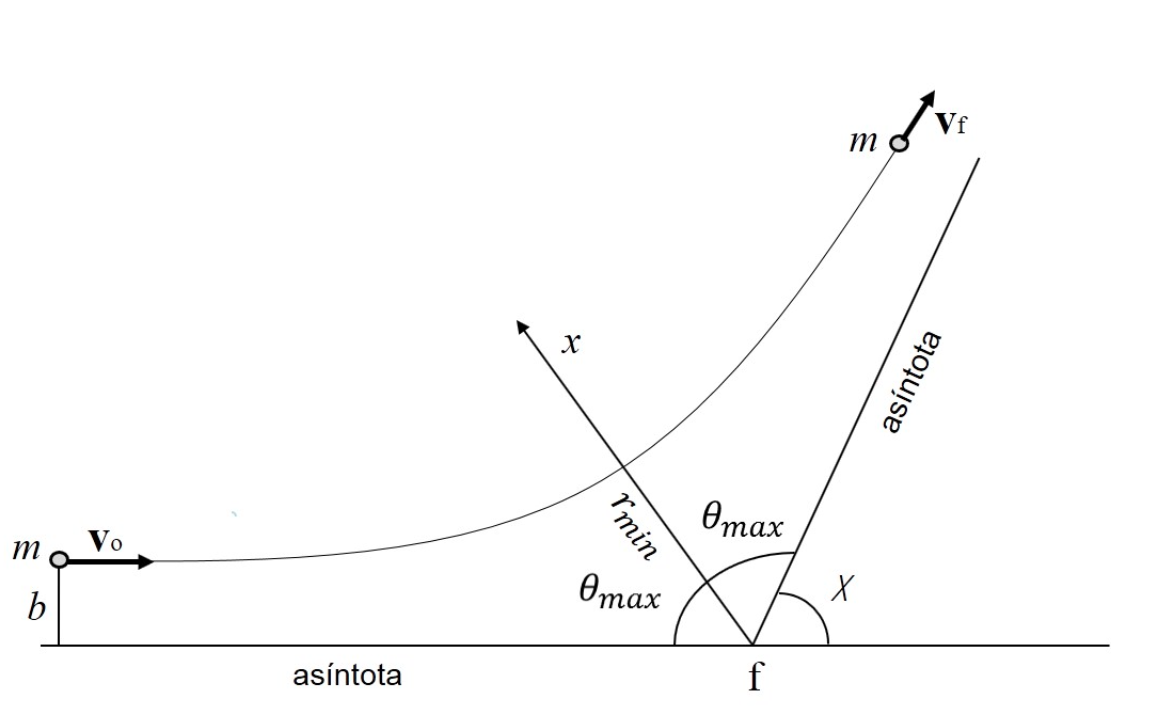
\includegraphics[width=1.8in]{Figuras/Dispersion.png}
   	\end{figure}
	\item<2-> Consideremos una part�cula de masa $M$ situada en el foco $f$ y una part�cula con masa $m \ll M(\mu \approx m)$ incidente desde $r \rightarrow \infty$
	\item<3-> La part�cula describe una trayectoria abierta desde $r=\infty$ hasta $r=r_{\min }$ y retorna a $r=\infty$, cambiando la direcci�n de su velocidad. 
	\item<4-> El �ngulo entre la direcci�n del vector velocidad inicial $\mathbf{v}_0$ y la direcci�n del vector velocidad final $\mathbf{v}_f$ se denomina �ngulo de dispersi�n, que denotaremos por $\chi$
    \end{itemize}
}
%
%%%%% Diapo 2
\section{Par�metro de Impacto}
\frame{
\frametitle{Par�metro de Impacto}
\begin{itemize}  
  	\item<1-> La energ�a inicial de la part�cula en $r=\infty$ es $E=\frac{1}{2} m v_0^2$ 
	\item<2-> El par�metro de impacto $b$ es la distancia perpendicular entre la direcci�n de la velocidad inicial $\mathbf{v}_0$ de la part�cula incidente y la recta paralela que pasa por el centro del potencial $V(r)$
	\begin{figure}[t]
		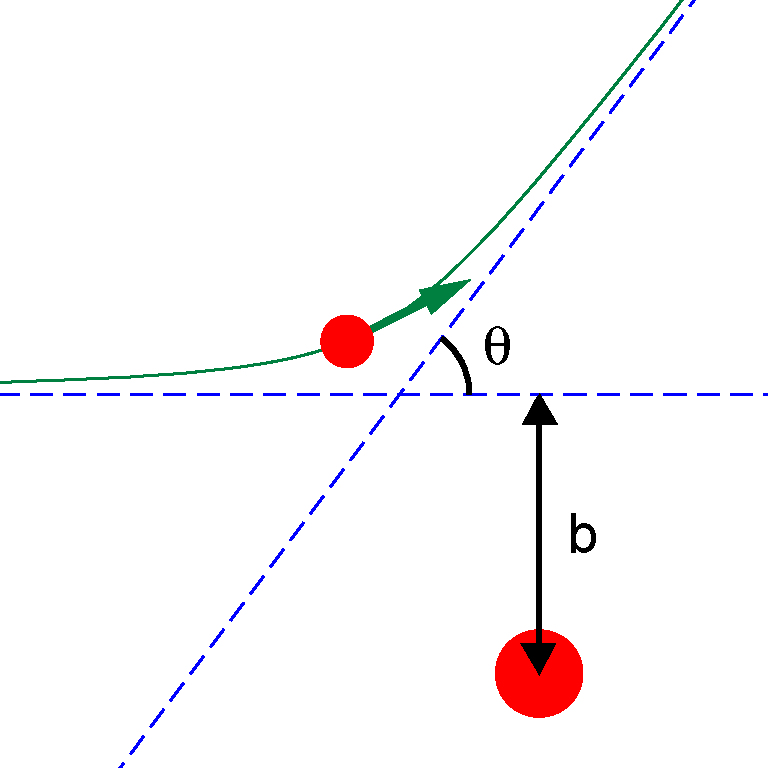
\includegraphics[width=1.5in]{Figuras/Impctprmtr.png}
   	\end{figure} 
	\item<3-> Los datos claves para la dispersi�n con campos centrales son $b$ y $E$.
\end{itemize}
}
%
%%%%% Diapo 2
\section{Dispersi�n Hiperb�lica}
\frame{
\frametitle{Dispersi�n Hiperb�lica}
\begin{itemize}  
	\item<1-> La magnitud del momento angular de la part�cula ser� $L=  r p \sin (\pi-\theta)=m v_0 r \sin \theta=m v_0 b \Rightarrow L^2=  m^2 v_0^2 b^2=2 E m b^2$
	\item<2-> Si  $V(r)=-\frac{k}{r}$, la �rbita con $E>0$ es una hip�rbola, $\frac{q}{r}=1+e \cos \theta$, con 
	$q  =\frac{L^2}{m k}=\frac{2 E b^2}{k}$ y $e =\sqrt{1+\frac{2 E l^2}{m k^2}}=\sqrt{1+\left(\frac{2 E b}{k}\right)^2}>1$
	\item<3-> Entonces: $r_{\min }  =\frac{q}{1+e}, \quad \text { para } \theta=0$ y $r_{\max } \rightarrow \infty \quad \text { para } \cos \theta_{\max }  =-\frac{1}{e} \Rightarrow \frac{\pi}{2}<\theta_{\max }<\pi$
	\item<4-> El �ngulo de dispersi�n $\chi$ entre las as�ntotas es $\chi=2 \theta_{\max }-\pi$.
	\item<5-> Esto es $\cos \left(\frac{\chi}{2}+\frac{\pi}{2}\right) =\cos \theta_{\max } \Rightarrow {\rm sen}\; \left(\frac{\chi}{2}\right) =\frac{1}{e}$
	\begin{figure}[t]
		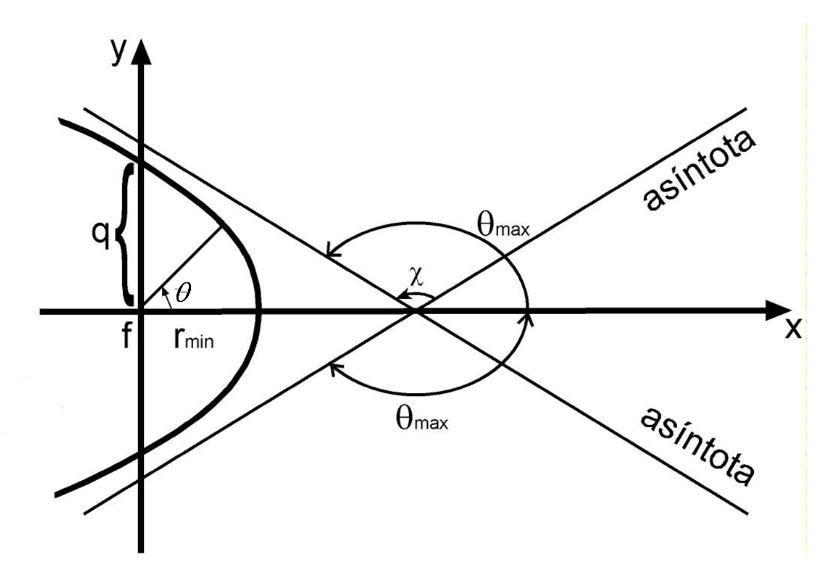
\includegraphics[width=1.5in]{Figuras/DispersionHiperbolica.png}
   	\end{figure} 
	\item<6-> Oumuamua \url{https://science.nasa.gov/solar-system/comets/oumuamua/}
\end{itemize}
}
%
%%%%% Diapo 2
\section{Secci�n}
\frame{
\frametitle{T�tulo transparencia}
\begin{itemize}  
	\item<1-> 
\end{itemize}
}
%
%%%%% Diapo 2
\section{Secci�n}
\frame{
\frametitle{T�tulo transparencia}
	\begin{itemize}  
\item<1-> 
    \end{itemize}
}
  
\end{document}
